\documentclass[10pt]{article}
\usepackage[a4paper, total={170mm, 257mm}]{geometry}

\usepackage[
backend=biber,
style=nature,
sorting=none
]{biblatex}
\addbibresource{References.bib}
%\bibliographystyle{unsrt}


\usepackage{amsmath}
\usepackage{amssymb}
\usepackage{upgreek}
\usepackage{dsfont}
\usepackage{esint} % various fancy integral symbols
\usepackage{mathrsfs} % for \mathscr

% fancy notation stuff
\usepackage{accents}
% vector arrows under the symbol to distinguish covariant and contravariant
\newcommand\undervec[1]{\underaccent{\vec}{#1}}

\usepackage{siunitx}
\DeclareSIUnit{\litre}{l} % litres as lower case l (upper case L by default)

%\usepackage{hyperref}

\usepackage{graphicx} % Required for inserting images
\usepackage{multicol}
\usepackage{mathpazo}
\usepackage[font=sf,labelfont=bf]{caption}

% title, headings, abstract heading in sans serif font and maybe color
%\usepackage{sectsty}
%\usepackage{titling}
%\usepackage[sf,bf,pagestyles]{titlesec}
\usepackage[dvipsnames]{xcolor}
\usepackage{sectsty}
\usepackage{abstract}
\renewcommand\abstractnamefont{\sffamily\bfseries}%\color{Maroon}}
%\chapterfont{\color{blue}}  % sets colour of chapters
\sectionfont{\sffamily}%\color{Maroon}}  % sets colour of sections
\subsectionfont{\sffamily}%\color{Maroon}}  % sets colour of subsections
\subsubsectionfont{\sffamily}  % sets colour of subsections





% TO DO's
\newcommand{\todo}[1]{ {\color{ForestGreen} [#1]} }

\graphicspath{{figures/}}

\usepackage{lipsum} 

% referencing commands
\newcommand{\seefig}[2]{\mbox{\sffamily($\rightarrow$ Fig. \ref{#1}#2)}}
\newcommand{\reffig}[2]{\mbox{\sffamily{Figure \ref{#1}#2}}}


\title{\sffamily\bfseries\color{Maroon} Scattering Spectroscopy of\\Plasmonic Janus Particles}
\author{Felix H. Patzschke and *Frank Cichos}
%\date{November 2023}
\date{}



\begin{document}
%\allsectionsfont{\sffamily}


\twocolumn[\maketitle \begin{abstract}\sffamily \vspace{-1em} 
%The light-matter interactions of plasmonic nanostructures are of great importance to [whom?].
%For plasmonic Janus particles in particular, which are established as an often-used tool in active matter research, the [???] is two-fold. [...]
%Metal-coated Janus particles have established themselves as a valuable tool in active matter research \cite{MONA-flow-fields} and related fields, owing to their plasmonically active nanostructures which allow for both excellent visibility in dark-field applications, as well as for efficient heating and, consequently, motility. \cite{MONA-thermotaxis, MONA-photon-nudging-1} 
%With light-matter interactions enhanced through their plasmonically active nanostructures, metal-coated Janus particles allow for both excellent visibility in dark-field applications as well as efficient heating and, consequently, motility \cite{MONA-thermotaxis, MONA-photon-nudging-1}, making them a valuable tool for active matter research. \cite{MONA-flow-fields}
%In recent years, theoretical predictions have been made of counter-intuitive optically enabled behaviours of such particles. \cite{Ilic2017}
%Nonetheless, these light-matter interactions are not yet thoroughly understood; in particular, there does not yet exist a proven method of inferring the out-of-image-plane orientation of a spherical Janus particle from its dark-field image. 
%Nonetheless, these light-matter interactions are not yet thoroughly understood.

%We present an experimental method for the orientation-dependent scattering spectroscopy of such anisotropic microscale particles. 
% $\SI{1}{\micro\meter}$ PS + $\SI{50}{\nano\meter}$ Au
%We analysed the scattering behaviour of \mbox{1µm PS + 50 nm Au} Janus Particles, resolving for wavelength, direction of illumination and scattering angle.
%under dark-field illumination and reproduced the results by finite-elements simulations. 
%We find well-discernible spectral features, particularly in the NIR range, that appear or disappear, depending on the orientation of the JP. 
%Further, we reproduced the experimental results by finite-element simulations.
%These findings may be worked into a method of determining the notoriously elusive out-of-plane orientation of spherical JPs, possibly even in real-time.

%We identify spectral markers, particularly in the near infrared range, that depend heavily on the orientation of the Janus particle; a result that may enable a new method of determining the notoriously elusive [to do: reference] out-of-plane orientation of spherical JPs, possibly even in real-time.
Plasmonic Janus particles consist of dielectric core particles with a thin metallic cap on one side and are widely used in active matter research. \cite{MONA-flow-fields} 
The plasmonic cap enhances optical scattering and absorption, allowing for self-propulsion through temperature gradients as well as efficient trapping and tracking. \cite{MONA-thermotaxis, MONA-photon-nudging-1} 
The asymmetry of such a particle gives rise to surface plasmon modes whose excitation is sensitive to the angle at which the particle is illuminated. 
Even though the angle of illumination strongly influences the particle's scattering response, the optical properties of such metallic caps have hardly been investigated. 

We probe the light scattering of individual micrometre-sized, spherical, Au-coated Janus particles by means of Selective Illumination Multiplexed Fourier Plane Spectroscopy. 
This novel method allows us to explore microparticles' scattering characteristics resolved for wavelength, angle of illumination and scattering angle. 

In addition, we supplement our experimental results with finite-element simulations and correlate spectral markers to orientation-dependent surface plasmon modes. 
This additional information on the correlation of angular and spectral information could pave the way for new methods of orientation detection. They also shed new light on the interaction of such spherically capped particles with light inducing forces and torques. \cite{Ilic2017, BA}
 \\ \end{abstract}]
%\begin{multicols}{2}


\section*{Introduction}

%\lipsum[1-3]

Janus particles (JPs) with a plasmonically active cap are a widely-used tool in active matter research: 
Through the absorption of visible light, the cap can be heated efficiently. 
In conjunction with the anisotropy of the particle, this facilitates directed self-propulsion. 
Meanwhile, the enhanced optical scattering of the cap leads to good visibility in microscopy, particularly in the dark field, which, in turn, allows for accurate tracking of the motile particles. 

\todo{However, orientation studies are usually performed in 2D, as ...}

As widely applicable as these particles' light-matter interactions (LMIs) may be, the are certainly not trivial: 
The length scales of the surface curvature are in the same order of magnitude as the wavelengths of light in the interaction, such that approximations along the lines of ray optics or dipole scattering are invalid. 
In addition, the asymmetry of the particles leads to orientation-dependency of the LMI. 
These orientation-dependencies may manifest in counter-intuitive ways: 
Some purely numerical studies suggest that plasmonic JPs can stably rotate, powered by a linearly polarized light field. \cite{Ilic2017,BA}

As a first step towards an understanding of such effects, we study the scattered light from these JPs. 
We measure scattering spectra of individual JPs while varying the direction of illumination as well as resolving for the scattering angle. 
%To our knowledge, this manner of LMIs has not yet been systematically studied. 
While orientation-dependent scattering studies of plasmonic nanostructures %\footnote{specifically, Au nano-rods and -triangles, sized between 100 and 150 nm} 
\emph{have} been performed, \cite{Islam2021} %neither has that been the case on JPs nor with a capacity for spectral resolution beyond RGB-decomposition. 
that has only been the case for Au nanostructures significantly smaller than the observation wavelengths. 
As such, no regard was given to the angular distribution of the scattered light. %\footnote{which on such small objects isn't necessary - the angular distribuions look pretty much the same - but for larger particles, the differences in the shapes of the Mie plots can lead to drastic differences between the "true" scattering spectra and the measured ones.} 
In our studies of micrometre-sized JPs in visible and NIR light though, we find that the difference in shape of these distributions can lead to drastic, qualitative differences in measured scattering spectra. 

We present an experimental method, which we use to study the LMI of plasmonic JPs consisting of a spherical polystyrene (PS) particle, $\SI{1}{\micro\meter}$ in diameter, with a $\SI{50}{\nano\meter}$ thick gold layer as the cap. 
We resolve the intensity of scattered light for wavelength and scattering angle. 
Though the theory of Mie \cite{Mie1908} only makes predictions for maximally symmetric particles, it serves well as reference in the characterization of the LMI of plasmonic JPs. 

We complement the measurement results with numerical simulations and find a good match between both methods' results. 
Through the analysis of the simulation results, we correlate peaks in the scattering spectra to orientation-dependent surface plasmon modes. 









\section*{Methods}





\begin{figure*}[htbp]
    \centering
    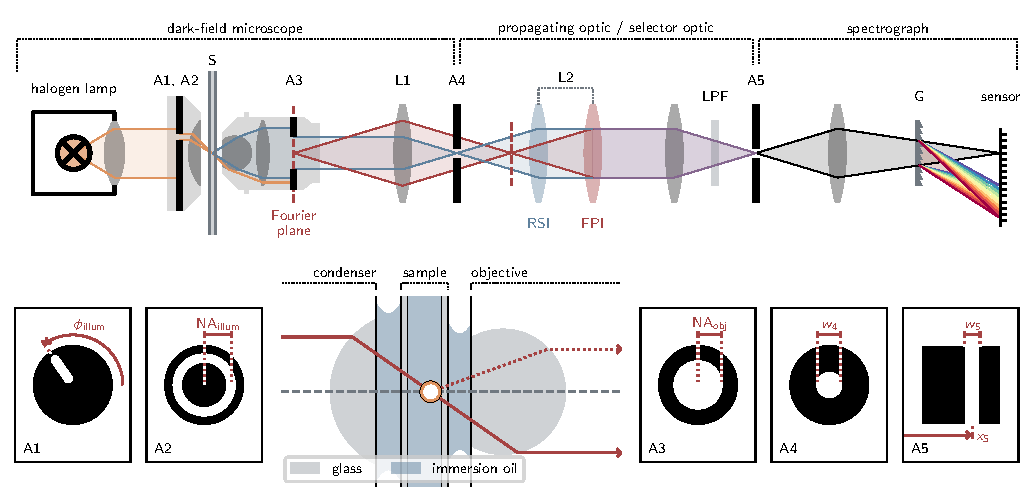
\includegraphics[width=\textwidth]{[fig] setup}
    %\includegraphics[width=\textwidth]{(fig) optics}
    \caption{
    %Schematics of the imaging optics: 
    {\sffamily\bfseries (top)} Imaging light path. %The dark-field condenser directs the illumination (yellow light path) onto the sample {\sffamily (S)}; the apertures {\sffamily A1} and {\sffamily A2} restrict the direction of illumination. 
    Schematics of the apertures ({\sffamily\bfseries A1-A5}) are shown below. 
    {\sffamily A4} lies in an image plane, {\sffamily A1-A3} lay in Fourier planes. Depending on the placement of {\sffamily L2}, either the image plane or the Fourier plane may be imaged onto {\sffamily A4}, and subsequently the camera sensor. 
    In the vicinity of the particle under observation {\sffamily\bfseries (bottom center)}, the ambient refractive index is virtually homogenous, due to the usage of immersion oil inside the sample.  
    }
    \label{fig:setup}
\end{figure*}

\subsection*{Experiments}

\subsubsection*{Sample Preparation}

The JPs consisted of spherical PS beads, coated with a layer of gold, $\SI{50}{\nano\meter}$ thick on average, on one side, with a $\SI{5}{\nano\meter}$ thick layer of chromium as a binding agent in between. 
A $\SI{30}{\micro\litre}$ droplet was placed on a cover slip and the JPs in solution were left to sediment for \mbox{10 minutes}. 
Afterwards, the solvent was blown off using nitrogen gas, leaving the remaining JPs stuck on the coverslide. 
A second cover slip was placed on top, with a droplet of $\SI{1.5}{\micro\litre}$ of immersion oil\footnote{\sffamily Immersol 518 F, Carl Zeiss Jena GmbH} in between, such as to keep the ambient refractive index constant in the vicinity of the particles.   

\subsubsection*{Optical Setup}

The imaging setup is sketched in \reffig{fig:setup}{C}. 
Its basis was formed by a standard dark-field microscope, constructed around an {\sffamily OLYMPUS IX71} microscope base. 
A confocal aperture in the image plane of the dark-field microscope was used to isolate an individual particle. 
A homebuilt spectrograph was used to extract spectral information from the microscope image. 
%It consisted of 
%%At the other end of the optical path stood a homebuilt spectrograph, consisting of 
%\begin{itemize}
%    \item an sCMOS camera \mbox{\sffamily(pco.edge 4.2)} for image acquisition, 
%    \item[{\sffamily(G)}] a transmissive diffraction grating {\sffamily(ThorLabs GTI25-03A)} in front of it, used for spectral dispersal of the image,
%    \item[{\sffamily(A5)}] a tunable slit to select only a thin vertical line from an image in order to prevent overlap of spectrally dispersed signals from different points in the original image and
%    \item a lens to propagate the image from the plane of the slit onto the camera sensor.  
%\end{itemize}
The microscope and spectrograph sub-assemblies were linked by a simple propagating optic, with which either the image plane wherein the aperture lay or the back focal plane (BFP) of the microscope objective could be chosen to be projected onto the slit {\sffamily(A5)}. 



The real-space-imaging mode was used to select particles for measurement as well as for spectral measurements in which the scattering angle was not resolved. 
The BFP-imaging mode was used to record spectrally resolved Fourier-space scattering maps of the JP under observation. 
To that end, the slit {\sffamily{A5}} was slowly translated across the BFP image while recording an image sequence, such that the camera would record one spectrally dispersed vertical line of the BFP image at a time. 
This step being the spatio-temporal multiplexing of the line-wise spectral signals, the corresponding de-multiplexing is done later, by appropriately re-arranging the intensity data from the image stack. 
\todo{This procedure is described in detail in the supplementary material and in \cite{MA}.} 
The accumulation time for one such dataset was approximately \mbox{15 minutes}. 

%The calibration data for the wavelength-dependent sensitivity of the optics was collected by allowing the illumination light to pass through the entire assembly and recording its spectrum. 
Measurements had to be corrected for the spectral response function of the setup. 
This was recorded by opening the objective's back aperture {\sffamily(A3)} fully, allowing the illumination light to pass through the entire assembly. 

\begin{figure}[h]
    \centering
    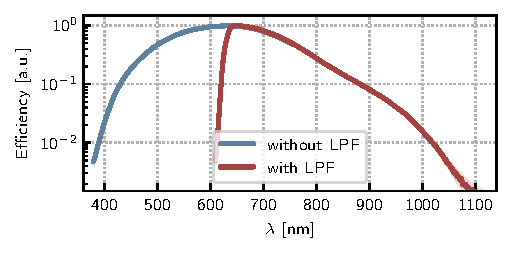
\includegraphics[width=\columnwidth]{corrections-log}
    \caption{Spectral efficiency of the optical setup.}
    \label{fig:corrections}
\end{figure}

The spectral efficiency of the setup, being the accumulated product of the lamps's emission spectrum, the camera's quantum efficiency and the optics' transmittivities, is illustrated in \reffig{fig:corrections}{}. 
We deem this sufficient for wavelengths between $\SI{400}{\nano\meter}$ and $\SI{1000}{\nano\meter}$. 

\note{I'm leaving out the laser for position calibration stuff. $\rightarrow$ supplement?}





\subsection*{Numerical Methods}

\subsubsection*{Definition of the Orientation}
 

In order to assure comparability between experimental and numerical results in terms of the orientation of the system, we define three unit vectors;  
%The orientation of the system is characterised by the angles between three unit vectors;
\begin{itemize}
    \item[$\hat{z},$] the symmetry axis of the particle, oriented such that the Au cap lies in the positive and the PS side in the negative $z$-direction, 
    \item[$\hat{k}_0,$] the propagation direction of the incident light, with respect to which scattering angles are defined and
    \item[$\hat{o},$] the "forward" direction along the optical axis, equivalent to the central axis of the objective's collection cone. 
\end{itemize}
In terms of these, the \emph{out-of-plane orientation} of the JP is defined as
$\alpha := \measuredangle( \hat{o}, \hat{z} )$.
Similarly, we define the \emph{illumination angle} 
$\zeta := \measuredangle( \hat{k}, \hat{z} )$. 
%, which, in this model, is the only orientation parameter needed to define the light-matter interaction of the JP. 

Scattering angles are defined for each plane-wave contribution to the scattered field: 
Let that contribution have a propagation direction $\hat{k}'$. 
Then, \mbox{$\theta := \measuredangle( \hat{k}', \hat{k} )$} is the \emph{polar} component of the \emph{scattering angle}. 
Additionally, there is an azimuthal component $\phi$, the choice of reference point for which being somewhat arbitrary. 
In the following, it will be chosen such that if $\hat{k}'$ lies in the $(\hat{k},\hat{z})$ plane, then $\phi=0$. 


These definitions are illustrated in \reffig{fig:vectors-and-angles}{}. 

\begin{figure}[htbp]
    \centering
    \begin{overpic}[width=1.0\columnwidth]{angles_sketch_larger_v2}
    % subplot label
    %\put (0,96) {{\sffamily\textbf{A}}}
    % vector labels
    \put (44,4) {$\hat{o}$}
    \put (0,31.5) {\textcolor{ts_y}{$\hat{z}$}}
    \put (0,67.5) {\textcolor{ts_b}{$\hat{k}_0$}}
    \put (77,6) {\textcolor{ts_r}{$\hat{k}'$}}
    % angle labels
    \put (60,74.5) {\textcolor{ts_b}{$\zeta$}}
    \put (33.5,27) {\textcolor{ts_y}{$\alpha$}}
    \put (30,80
    ) {{$\theta_o$}}
    \put (69,32) {\textcolor{ts_r}{$\theta$}}
    \end{overpic}
    \caption{
        %{\sffamily\textbf{A:}} 
        Unit vectors and angles defining the orientation of the system. 
        %{\sffamily\textbf{B:}} 
        %\todo{Integration domain corresponding to the objective aperture.} 
    }
    \label{fig:vectors-and-angles}
\end{figure}


\subsubsection*{Finite-Element Simulation}



The finite-element simulations were performed in COMSOL \mbox{Multiphysics 6.1}. 
%The simulation per se is ignorant of real-world optical devices and.
%Therefore, the geometric definition of the model does not depend on \mbox{$\hat{o}$-direction} or the objective aperture. 
\todo{Reference that the COMSOL model is qualitatively the same as in \cite{BA}.} 

The model was set up as follows: 
A polystyrene (PS) sphere ($r=\SI{0.5}{\micro\meter}$), centered at the origin, represents the core of the JP. 
The gold cap is modelled as half of an ellipsoidal shell around the PS sphere, cut off in the $z=0$ plane. 
Its semi major axis is parallel to $\hat{z}$ with a length of $\SI{0.55}{\micro\meter}$, its semi minor axes with length $\SI{0.51}{\micro\meter}$ lie in the $(x,y)$ plane.\footnote{$\hat{x},\hat{y},\hat{z}$ form a right-handed orthonormal basis of $\mathds{R}^3$.} 
This gives a thickness of $\SI{50}{\nano\meter}$ at the apex and a width of $\SI{10}{\nano\meter}$ to the rim. 
%The ellipsoid is cut off in the $(x,y)$ plane of the minor axes, its major axis coincides with the symmetry axis of the JP. 
%The particle model is surrounded by an ambient medium with a constant, real-valued refractive index. 
%The model geometry, based on models E1 and E2 from \cite{BA}, was defined in particle-coordinates, i.e. $\hat{z}$ coincides with the $z$-axis and $\hat{k}$ lies in the $xz$ plane. 
\todo{sketch?}

For the complex refractive index of gold, the values by Johnson \& Christy \cite{Johnson1972} were used. 
The medium surrounding the particle was modelled with a refractive index of $1.51$ to mimic the immersion oil used in the experiments. 

As parameters, the simulation takes in the illumination angle $\zeta$ and the incident (vacuum-)wavelength $\lambda$, such that
$$
    \vec{k}_0 = \frac{2\pi \mathfrak{n}}{\lambda} \left( \cos\zeta \cdot \hat{z} + \sin\zeta \cdot \hat{x} \right)
$$
is the wave vector of the incident light field. 

From the numerical solution to Maxwell's field equations for each fixed parameter vector, the far-field intensities $\mathrm{d}\mathcal{I} ~:~ \mathcal{S}^2 \ni \Omega \mapsto \mathrm{d}\mathcal{I}(\Omega)$ of the scattered field and the scattering cross-section $\sigma_\mathrm{sca}$ are calculated. 






\subsubsection*{Selective Integration}

%In order to be able compare the simulation results to the measurements, the the limited collection angle of the objective has to be taken into account. 

In the experiment, scattered light can only contribute to recorded scattering signals if it is collected by the objective. 
While the "true" scattering intensity is the integral over the angular distribution of scattered light, 
$$
    I_\mathrm{sca} = \oiint_{\mathcal{S}^2} \,\mathrm{d}\mathcal{I}(\Omega) \ , % \ \mathrm{d}\Omega \ ,
$$
the measured value corresponds to the integration over a certain angular range, % $\mathcal{D} \subset \mathcal{S}^2$: 
$$
    I_\mathrm{sca,measured} = \iint_{\mathcal{D}} \,\mathrm{d}\mathcal{I}(\Omega) \ , 
$$
where $\mathcal{D} \subseteq \mathcal{S}^2$ is the set of propagation directions $\hat{k}'$, for which a plane wave component will pass through the objective aperture. %contribute to the signal on the detector. 
Specifically, $\mathcal{D}$ is the interior of a small circle which is centered around $\hat{o}$ and whose angular radius $\rho$ is defined by the numerical aperture of the objective, 
$$
    \rho = \mathrm{asin}\!\left( \frac{\mathrm{NA}_\mathrm{obj}}{n_\mathrm{oil}} \right) \ ,
$$
according to the Abbe sine condition. \cite{MONA-BFP-photonic-crystals,MONA-BFP-photonic-stop-bands} \todo{Sketch!}
Analytically, this requirement can be formulated as 
$$
    \mathcal{D} = \left\lbrace\ \hat{k}' \in \mathcal{S}^2\ \middle\vert\ \measuredangle\!\left( \hat{k}', \hat{o}\right) < \rho\ \right\rbrace
    \ .
$$

%In the experiment, $\hat{o}$ and $\theta_o$ are fixed, and $\hat{k}_0$ is a known parameter. 
%In the simulation, $\hat{z}$ is fixed instead, while $\zeta$ (and thus $\hat{k}_0$) is varied. 

As the objective is not considered in the simulations of the scattering process per se, appropriate values for $\hat{o}$ and $\mathrm{NA}_\mathrm{obj}$ have to be chosen now, in order to emulate an experiment: 
%We first choose a fixed $\alpha$ and then compute a sampling of pairs $\left( \hat{k}'_0 , \hat{o}' \right) \in \left. \mathcal{S}^2 \right\vert_{y=0} \times \mathcal{S}^2$, such that 
We first choose a fixed $\alpha$ and then compute a sampling of pairs $\bigl( \hat{k}'_0 , \hat{o}' \bigr) \in \mathcal{S}^1_{xz} \times \mathcal{S}^2$, such that 
$$
    \measuredangle\!\left(\hat{z} , \hat{o}'\right) = \alpha
    \quad \text{and} \quad 
    \measuredangle\!\left(\hat{k}'_0 , \hat{o}'\right) = \mathrm{asin}\!\left( \frac{\mathrm{NA}_\mathrm{DFC}}{n_\mathrm{oil}} \right) 
    \ . 
$$
%the angle between the optical axis and the illumination cone from the dark-field condenser. 
We then choose the simulation datasets corresponding to the illumination angles defined by $\hat{k}'_0$ and the fixed $\hat{z}$ and integrate the far-field intensities over the domains $\mathcal{D}$ defined by $\hat{o}'$ and $\mathrm{NA}_\mathrm{obj}$, accumulating the results over all pairs $\bigl( \hat{k}'_0 , \hat{o}' \bigr)$.

%The end result of the selective integration is a sampled map 
This algorithm of selective integration yields a sampled map 
$$
    \alpha,\mathrm{NA}_\mathrm{obj} \mapsto \bigl[ \lambda \mapsto I_\mathrm{sca,measured} \bigr] \ ,
$$
where each $\bigl( \alpha, \mathrm{NA}_\mathrm{obj} \bigr)$ encodes a possible configuration of the system and $\lambda \mapsto I_\mathrm{sca,measured}$ is the measured scattering spectrum resulting from that configuration.  
%i.e. a scattering spectrum $\lambda \mapsto I_\mathrm{sca,measured}$ as measured for each sampled $\alpha,\ \mathrm{NA}$. 

%\begin{itemize}
%    \item The simulation provides values of the scattered field for sampled values of $\zeta$.
%    \item The numerical aperture of the dark-field condenser defines $\measuredangle(\hat{k},\hat{o})$.
%    \item The out-of-plane angle $\alpha$ of the JP is unknown and not uniquely defined by $\zeta$ and $\measuredangle(\hat{k},\hat{o})$. We sample $\alpha\in\left[0,\pi\right]$ and weight the results by $p(\alpha) = \sin\alpha$.\footnote{$p(\alpha)$ is the probability density function for the out-of-plane angle of a randomly oriented spherical JP. For the derivation, see the supplementary material.}
%\end{itemize}









\section*{Results}

\subsection*{Validation}

%\subsubsection*{Validation}

%In order to validate the experimental setup, we recorded scattering data that could be compared to the predictions of Mie theory \cite{Mie1908, BohrenHuffman, GouesbetGrehan}. 

In order to validate the experimental setup, the scattering spectra of $\SI{65}{\nano\meter}$ AuNPs were measured. 
In \reffig{fig:AuNP}{A}, the measured scattering spectra are shown together with the prediction from Mie theory \cite{Mie1908}, computed using the values by Johnson \& Christy \cite{Johnson1972} for the complex refractive index of gold. 

\begin{figure}[htbp]
    \centering
    %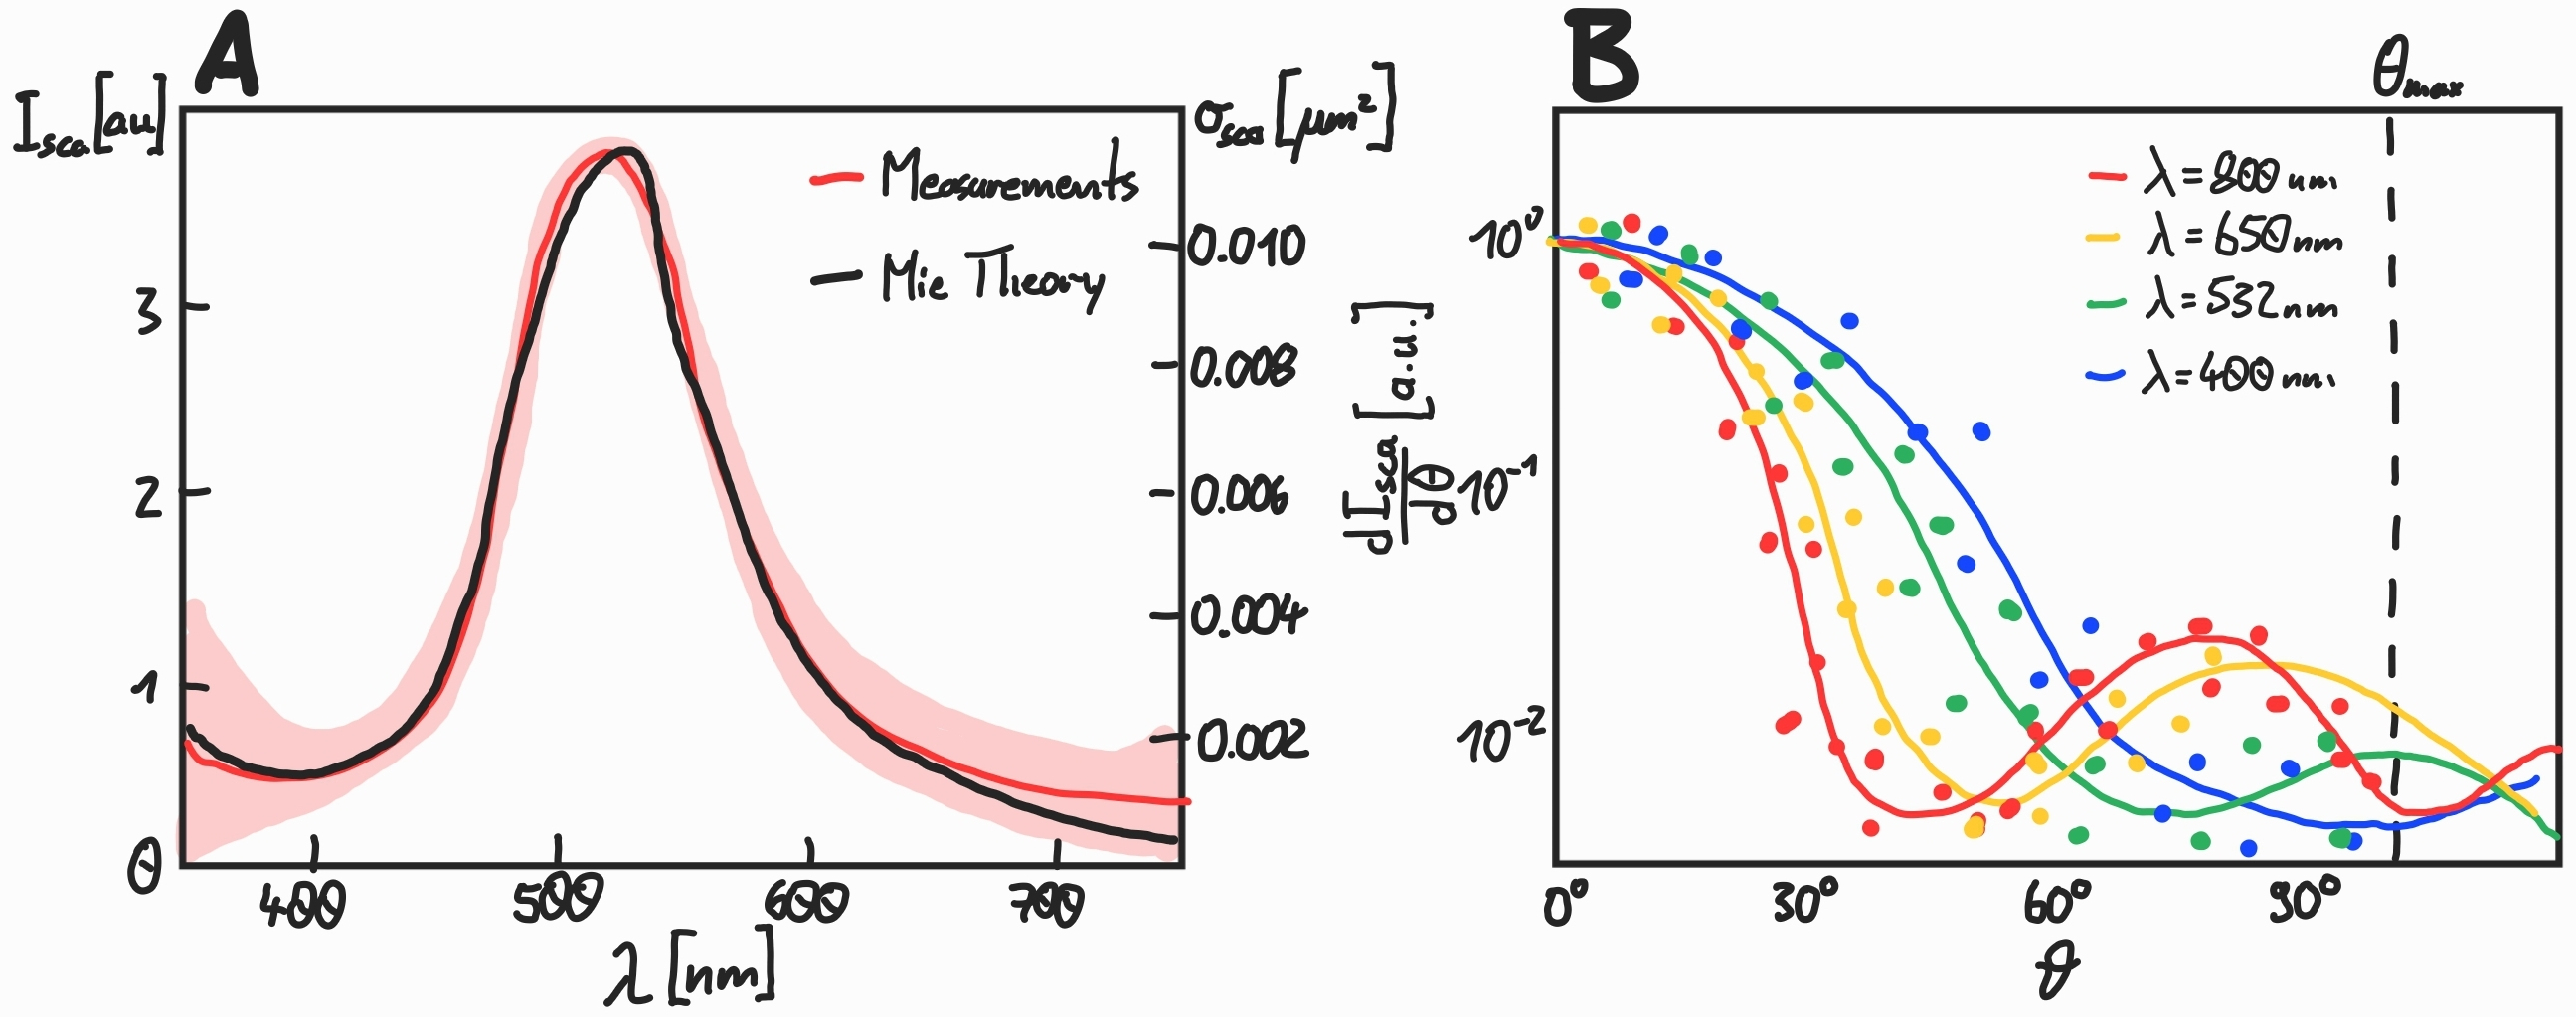
\includegraphics[width=\textwidth]{[fig] AuNP (placeholder).jpg}
    \begin{overpic}[width=\columnwidth]{AuNP Spectra}                           \put (6.5,50) {{\sffamily\textbf{A}}} \end{overpic}
    \begin{overpic}[width=\columnwidth]{[subfig] Mieplots-rect-thcomp-Au250-SP} \put (8,50)   {{\sffamily\textbf{B}}} \end{overpic}
    \caption{Validation measurements. 
    {\sffamily\bfseries A:} 
    Scattering spectrum of \mbox{65 nm} Au NPs. The shaded area corresponds to the maximum noise in the measurements. 
    {\sffamily\bfseries B:} 
    Scattering intensity of a spherical Au NP \mbox{(d = 250 nm)} versus the scattering angle for various wavelengths. 
    The lines show the predictions of GLMT \cite{GouesbetGrehan}, scaled by a constant factor to match the points showing the measurement results. 
    }
    \label{fig:AuNP}
\end{figure}

%In the comparison of the measured spectra to the predictions of Mie theory \cite{Mie1908, BohrenHuffman, GouesbetGrehan} using the values by Johnson \& Christy \cite{Johnson1972} for the complex refractive index of gold shows a strong agreement. 

We decided on the use of these much smaller particles because the expected resonance peak in the scattering spectrum would be as narrow as possible, giving a good indication as to the spectral resolution of the measurement. 
Furthermore, the shape of the angular distribution of scattered light would not change appreciably over the spectral range of interest, causing the measured and full scattering cross-sections to only differ by a constant factor. 

We find a good match between the measured and theoretical spectra. 
%This is, in part, due to our choice of particles: 
As the particles were significantly smaller than any wavelength considered, the scattered field is well-approximated by a dipole field. 
%The approximately constant shape of the angular intensity distributions meant that the fraction of scattered light being collected by the objective would also be approximately constant over the measured spectral range.
Still, the shift of the measured scattering peaks towards the red end of the spectrum, caused by the slightly flatter intensity distribution at longer incident wavelengths is significant.

%For the larger JPs, the comparison of measured and simulated spectra would necessitate a correction for the differing distributions. 

%For the larger JPs, it would be necessary to correct for the differing distributions. 
To test the BFP spectroscopy, we chose larger Au particles ($d=\SI{250}{\nano\meter}$). 
The results are shown and compared to the predictions of GLMT\footnote{Generalized Lorentz-Mie Theory}\cite{BohrenHuffman, GouesbetGrehan} in \reffig{fig:AuNP}{B}. 
Again, we find good agreement between experiment and theory. 

The choice of these larger particles is due, first and foremost, to their much greater brightness in the dark field: 
In the BFP measurement, the scattered light is distributed over a larger area on the sensor, lowering the SNR. 
The greater scattering cross-section of larger particles remedies that issue. 
Nonetheless, the scattering cross-section of one such AuNP could be expected to be smaller than that of a JP as used later-on, implying that if the measurement was valid for the AuNPs, it would also be for the JPs. 
In addition, with a size close to the wavelengths under consideration, a perceptible change to the angular intensity distributions could be expected. 
%\begin{enumerate}[label=(\alph*)]
%    \item as, in the BFP measurement, the scattered light is distributed over a larger area on the sensor, lowering the SNR. The greater scattering cross-section of larger particles remedies that issue. 
%    \item Moreover, with a size close to the wavelengths under consideration, a perceptible change to the angular intensity distributions could be expected. 
%    \item Nevertheless, the scattering cross-section of one such AuNP could be expected to be smaller than that of a JP as used later-on, implying that if the measurement was valid for the AuNPs, it would also be for the JPs. 
%\end{enumerate}





\subsection*{Dark-Field Spectra}




Recorded scattering spectra of the JPs are shown in \reffig{fig:spectra-measured}, along with numerical predictions. 
The results from both methods agree reasonably well, with the measured curves falling within a standard deviation of the average\footnote{\todo{explain that average}} of the numerically obtained spectra for the most part. 

\begin{figure}[h]
    \centering
    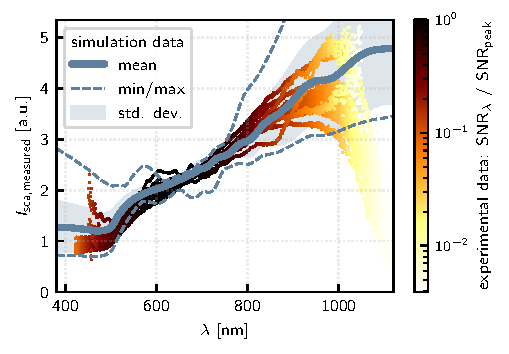
\includegraphics{[fig] spectra (measured).PDF}
    \caption{Measured scattering spectra (orange) atop value range as determined by simulation + emulation (blue).}
    \label{fig:spectra-measured}
\end{figure}

\begin{figure*}[htbp]
    \centering
    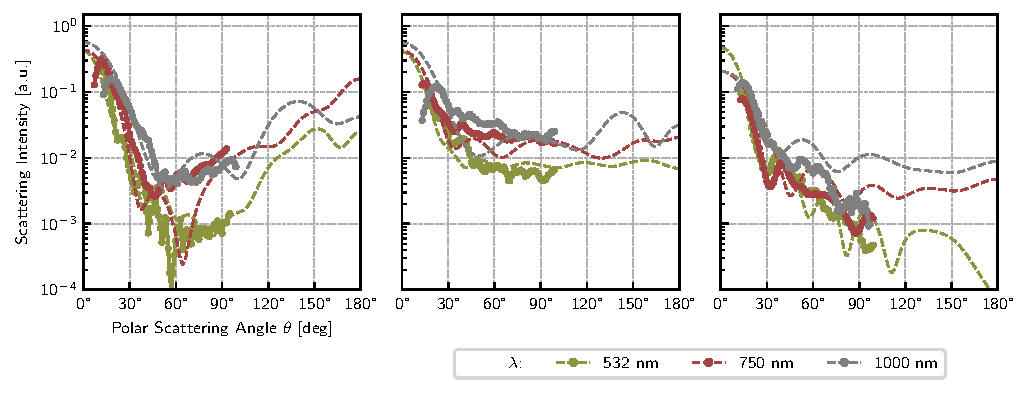
\includegraphics[width=\textwidth]{[fig] cartesian mieplots}
    \caption{Scattering intensity of the JP versus scattering angle for various wavelengths. 
    The points correspond to measured intensities while the lines are simulation results. 
    {\sffamily\bfseries A:} PS side illumination. 
    {\sffamily\bfseries B:} Au side illumination. %show the cylindrically symmetric cases of illumination from the PS side and from the Au side, respectively, i.e. where $\hat{k}\parallel\hat{z}$. 
    {\sffamily\bfseries C:} side-on illumination. %, the light is incident side-on ($\hat{k}\perp\hat{z}$, $\zeta=\pi/2$). 
    %Disregarding the local extrema, qualitatively distinct large-scale behaviour is apparent: Under illumination from the PS side {\sffamily\bfseries (A)}, the scattering intensity becomes globally minimal in the sideways direction. 
    %Meanwhile, under illumination from the Au side {\sffamily\bfseries (B)}, it reaches a plateau and under side-on illumination {\sffamily\bfseries (C)}, the scattering intensity drops consistently between forwards and backwards.  
    }
    \label{fig:jp-mieplots-oneline}
\end{figure*}

%\todo{Broad behaviour: Intensity of the scattering signal increases with wavelength.}

All spectra show a sharp upward bend at $\SI{500}{\nano\meter}$, the same as can be seen in the scattering spectra of similar-sized Au spheres. 
For longer incident wavelengths, we generally observe the scattering intensity to monotonously increase. 

Between $900$ and $\SI{1000}{\nano\meter}$, the degraded efficency of the measurement setup causes the relative influence of bleed light and sensor noise to increase, rendering the measurements increasingly unreliable.\footnote{\note{I'm using the word "increase" too often, but I can't come up with anything else.}} 
Hence, the measured spectra diverge from one another. 
The numerical results suggest that the trend of approximately linear increase should continue. 

Consistent between all measurements, there is a bump at $\SI{550}{\nano\meter}$. 
%This is, notably, the same wavelength as the main peak of an arbitrarily small AuNP's scattering spectrum. 
We attribute this to the LSPR of gold, though the otherwise increasing characteristic of the spectra diminishes the distinct peak that it would produce in the scattering spectra of small AuNPs into a mere bump. 

Neither in the measured, nor in the numerically obtained spectra were we able to discern any obvious features that we could relate to an orientational parameter of the system. 










\subsection*{Dark-Field Spectra under Selective Illumination}

\begin{figure}[h]
    \centering
    \begin{overpic}[width=0.2425\columnwidth]{[subfig] tomography 165deg}  \put (11,75) {\textcolor{white}{\sffamily\textbf{A}}} \end{overpic}
    \begin{overpic}[width=0.2425\columnwidth]{[subfig] tomography 113deg}  \put (11,75) {\textcolor{white}{\sffamily\textbf{D}}} \end{overpic}
    \begin{overpic}[width=0.2425\columnwidth]{[subfig] tomography -121deg} \put (11,75) {\textcolor{white}{\sffamily\textbf{E}}} \end{overpic}
    \begin{overpic}[width=0.2425\columnwidth]{[subfig] tomography 7deg}    \put (11,75) {\textcolor{white}{\sffamily\textbf{J}}} \end{overpic}
    % next line
    \begin{overpic}[width=0.2425\columnwidth]{[subfig] tomography 172deg}  \put (11,75) {\textcolor{white}{\sffamily\textbf{B}}} \end{overpic}
    \begin{overpic}[width=0.2425\columnwidth]{[subfig] tomography 85deg}   \put (11,75) {\textcolor{white}{\sffamily\textbf{F}}} \end{overpic}
    \begin{overpic}[width=0.2425\columnwidth]{[subfig] tomography -88deg}  \put (11,75) {\textcolor{white}{\sffamily\textbf{G}}} \end{overpic}
    \begin{overpic}[width=0.2425\columnwidth]{[subfig] tomography -8deg}   \put (11,75) {\textcolor{white}{\sffamily\textbf{K}}} \end{overpic}
    % next line
    \begin{overpic}[width=0.2425\columnwidth]{[subfig] tomography -157deg} \put (11,75) {\textcolor{white}{\sffamily\textbf{C}}} \end{overpic}
    \begin{overpic}[width=0.2425\columnwidth]{[subfig] tomography -41deg}  \put (11,75) {\textcolor{white}{\sffamily\textbf{H}}} \end{overpic}
    \begin{overpic}[width=0.2425\columnwidth]{[subfig] tomography 32deg}   \put (11,75) {\textcolor{white}{\sffamily\textbf{I}}} \end{overpic}
    \begin{overpic}[width=0.2425\columnwidth]{[subfig] tomography -27deg}  \put (11,75) {\textcolor{white}{\sffamily\textbf{L}}} \end{overpic}
    \caption{Dark-field images of a JP under selective illuminations. The respective in-plane angles are noted in the lower left corner.}
    \label{fig:tomography}
\end{figure}

\todo{Particle appears much brighter when illuminated from the Au side. It stands to reason that its out-of-plane orientation made it such that when the aperture was rotated such that the PS side would be illuminated, the light \emph{actually} hit side-on. (I.e. cap pointing ca. 30° up towards the condenser)}

With the selective illumination mode, we demonstrate the dependence of the JP's scattering intensity on the propagation direction of the incident light. 
\todo{need to have another look at the data} 




\subsection*{Fourier Plane Spectra}

In the multiplexed Fourier plane spectroscopy, the angular distributions of the scattering intensity became visible. 
%We considered three settings of the selective illumination: 
%\begin{itemize}
%    \item illumination from the Au side, i.e. maximal $\zeta$,
%    \item illumination from the PS side, i.e. minimal $\zeta$ and
%    \item side-on illumination, i.e. $\zeta \approx \pi/2$.
%\end{itemize}
We performed measurements under three different settings of the selective illumination, each chosen to match as closely as possible the cases of Au-side, PS-side and side-on illumination. 
Because the exact out-of-plane angle of the particle under observation is unknown and in order to allow for easier comparison of measured and numerical data, we extracted 1-dimensional intensity profiles along the polar coordinate from the Fourier plane images. 
Measured and simulated scattering profiles are shown in \reffig{fig:jp-mieplots-oneline}{}.  

For all illumination directions, most of the scattered light is only lightly deflected off of the propagation direction of the incident light. 
However, there were qualitative distinctions between the distributions that hold over the entire spectral range under consideration:
The peak brightness was highest for illumination from the Au side, while a wider peak and significant sideways scattering accumulated into a greater absolute brightness under illumination from the PS side. 

The behaviours described also hold true for the full images. 

Unsurprisingly, the distributions were symmetric about the axis of illumination. 
This was not the case for the side-on illumination, where light was preferentially scattered in the direction of the Au side. 



%\todo{Tighter focusing vs. isotropic baseline for Au- vs. PS side illumination + simulation shows the same}

%In addition to dependencies on the illumination angle and wavelength, 




%We conducted numerical simulations of the scattering of light by an individual JP. 
%From the solutions for the electromagnetic field, we computed observable quantities that correspond to those measured in the experiments. 

The simulated far-field patterns show the same results. 




\subsection*{Scattering Spectra}

Using the real-world optical setup, it is not possible to capture all of the scattered light. 
Yet, from the simulations, we can readily extract predicted values of the scattering cross-section of the JP: 
With the illumination angle as a parameter, we obtain a family of scattering spectra:
$$\zeta \mapsto \bigl[ \lambda \mapsto \sigma_\mathrm{sca} \bigr] \ ,$$ 
each spectrum $\lambda\mapsto\sigma_\mathrm{sca}$ corresponding to a specific illumination angle $\zeta$. 
%\todo{We only consider the scattering spectra for illumination directly from the Au side, from the PS side and side-on, for now. (And possibly the orientation-average curve)}
\reffig{fig:spectra-principal}{} shows the scattering spectra for the maximally symmetric orientations of $\zeta = 0$ and $\zeta = \pi$, as well as for $\zeta = \pi/2$, i.e. the case wherein $\hat{k}_0 \perp \hat{z}$. 
A scattering intensity map, taking into account other sampled illumination angles is shown in \todo{supplementary figure}.\footnote{\note{leaving this out, not because the other spectra would be trivial combinations of the principal ones (they're not), but because a discussion of those would entail a decomposition into the underlying effects, which (a) would neccessitate finding them in the high-symmetry cases first and (b) is outside the scope of this work.}} 

\begin{figure}[h]
    \centering
    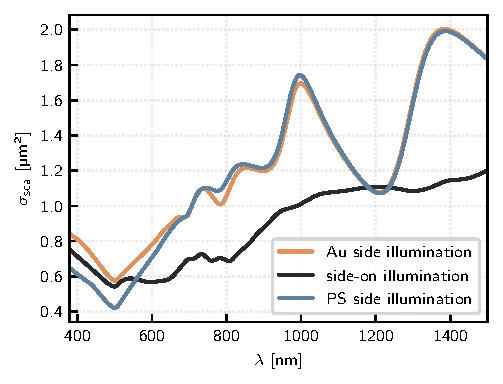
\includegraphics{[fig] spectra (principal).PDF}
    \caption{Simulated scattering spectrum of the JP under illumination from the Au side (yellow), from the PS side (blue) and from the equatorial side (black).}
    \label{fig:spectra-principal}
\end{figure}

The scattering spectra differ signifiantly from the measured dark-field spectra, though some correspondences between features can be inferred: 
The previously noted increasing trend is, once again, present, as is the sharp upward bend at $\SI{500}{\nano\meter}$. 
However, 
\todo{distinct wobbles for $\lambda > \SI{600}{\nano\meter}$, decrease of scattering cross-section up to the minimum at 500 nm} 

Within the visible part of the spectral range, the increase of the scattering cross-section coincides with that of the measured intensities. 
In the NIR range, the measured brightness increases further; this is due to the broadening of the forward scattering peak. 

For wavelengths beyond $\SI{700}{\nano\meter}$, the scattering cross-sections, between illumination from the Au side and from the PS side, are virtually the same. 
They are, moreover, significantly larger than that for side-on illumination, on average. 
However, at $\lambda=\SI{1210}{\nano\meter}$, they have a local minimum where the scattering cross-section is less than that for side-on illumination. 
This points at a polar plasmon mode that is being excited out-of-phase. 
\todo{Explain better what I mean.}
\note{Curiously, the peaks in the absorption spectra don't line up with either the valleys or the peaks in the scattering spectra. 
They don't for AuNPs either.}



This is due to only scattered light which is emitted in such a direction that it is collected by the objective contributing to the measured scattering intensity, while the simulated scattering spectra take into account the energy flow density of the scattered field itself. 














\section*{Discussion}

\subsubsection*{Spectra}

\note{The average of }\footnote{\note{most of the individual sample spectra fit reasonably well but there are some outliers. The average fits nicely, but ultimately one of those samples is likely the truth. And they have the same limitations in regards to details lost.}} 
The thus computed spectra reproduce the measured dark-field spectra well. 
Meanwhile, details such as the local maxima of the full scattering spectra are lost. \todo{with the possible exception of a small wobble at 850 nm, but it's unclear how exactly it arises. Maybe it's the $k=\pm 4$-peak?}


\todo{We find that the scattering cross-section heavily depends on the orientation of the JP.}
Over the spectral range that we analyzed, though decidedly not in general, the scattering efficiency of the particle was ... greater if it was illuminated from either the Au or the PS side than if it was illuminated side-on. 
In both cases, the scattering spectra have multiple peaks. 
Between axial and side-on illumination, though, there is no clear correspondence between these peaks. 

E.g., for side-on illumination, there is a scattering peak at $\lambda\approx\SI{550}{\nano\meter}$, that has no counterpart in the spectra for axial illumination. 
We ascribe this peak to the nanostructure plasmon resonance of gold: 
%It would be analogous to the spectrum of a small\footnote{tens of nanometres} Au particle added on top of the otherwise quite featureless spectrum of the JP. 
It sits right around that wavelength and it is only under side-on illumination that the incident electric field may be perpendicular to the surface of the Au cap at its points of highest curvature, that being the cap's perimeter. 

The bump at $\lambda\approx\SI{550}{\nano\meter}$ is discernable in both real and emulated measurements, while only appearing in the raw scattering cross-sections for side-on illumination. 
Notably, this peak occurs at the same wavelength as the main LSPR for an arbitrarily small AuNP. 
We reason that this plasmon is excited in the rim of the cap by electric fields that are perpendicular to the Au surface in its regions of maximal curvature. 

Conversely, the peak at $\lambda\approx\SI{996}{\nano\meter}$ is present under just the opposite circumstances, i.e. when $\hat{k}\parallel\hat{z}$. 
For these orientations, the system is rotationally symmetric in the polarization average and the surface plasmon propagates along the polar direction on the Au cap, inward for $\zeta=0$ and outward for $\zeta=\pi$. 
%Under excitation with $\lambda\approx\SI{996}{\nano\meter}$, the surface charge density changes its sign three between the apex and the rim. 
A quantity akin to a wave vector can be assigned to the polar surface plasmon mode, by counting the sign changes of the surface charge density on a geodesic path from the apex of the cap to its rim. 
For the $\SI{996}{\nano\meter}$ peaks, this means $\tilde{k}=\pm3$. 
\todo{Similarly, we can assign such a pseudo wave vector to all the other peaks in the scattering spectra for axial illumination. The result is \reffig{fig:polar-plasmon-modes}{}.}

\todo{Proper analysis of the surface plasmon wavevector stuff.}

\begin{figure}[htbp]
    \centering
    %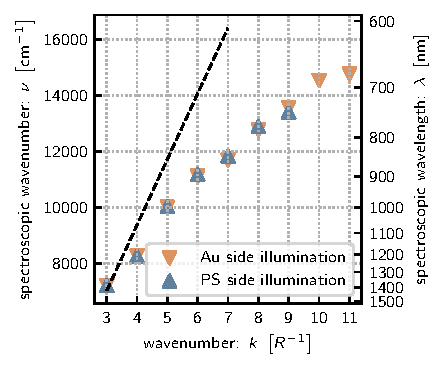
\includegraphics[width=\columnwidth]{[fig] polar plasmon dispersion relation}
    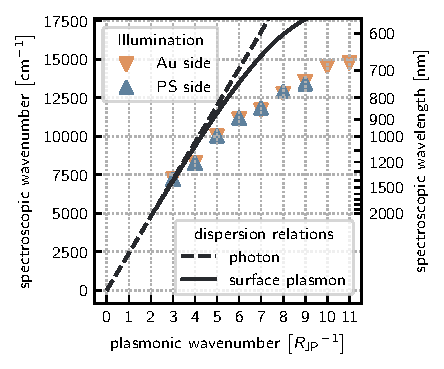
\includegraphics[width=\columnwidth]{[fig] SP dispersion relation + polar resonance}
    \caption{
        Excitation wavelengths of peaks and valleys in the axial illumination scattering spectra vs. spatial frequency of the electric field on the surface of the Au cap. 
    }
    \label{fig:polar-plasmon-modes}
\end{figure}

Neither of these peaks is present\footnote{discernable?} in the scattering spectrum of an equivalently sized Au sphere. 
This implies that \todo{either} the associated surface plasmon modes do not exist on a closed sphere in this form \todo{or the $\mathrm{Au}\mathcal{S}$ spectrum is more closely related to the orientation-average of the JP spectra than it is to any single one of them}. 

\todo{peaks and valleys correspond to only peaks on AuNPs $\rightarrow$ proximity of peaks makes them unresolvable}

The weak scattering of even-numbered resonances is due to the surface charge density having opposite signs in corresponding areas of the inside and outside of the gold cap. 
Whether the same effect could be observed on a core-shell particle of equivalent size is unclear: 
On one hand, it has been suggested that light interaction properties of JPs can be approximated as a mix between those of solid particles and of core-shells \todo{Citation: black paint}. 
On the other hand, visual inspections of the time-dependent solutions for the electric field suggest that the surface charge densities on the in- and outside of the cap are coupled via the boundary of the cap rather than through transmission through it. 
This would imply that the odd-even splitting would not happen on a CS particle, as transmission through the Au layer would be the only possible way of coupling the inside field to the outside one. 


\todo{For side-on illumination but arbitrary polarization, there is also something happening on the cap, not just on the rim. 
Would that be an extra class of modes? (let's call 'em longitudinal to distinguish them from the polar and azimuthal modes)
And are those the tiny peaks in the side-on scattering spectrum between 650 and 850 nm?}

Comparing the angular distributions to those of a Mie particle though, there is clear similarity: 
Non-global maxima become more well-distinguished and fewer in number as wavelength increases. 
%This is the expected behaviour in the transition from the ray optics regime $\left( \lambda \ll R \right)$ to dipole model $\left( \lambda \gg R \right)$. 
The same happens as the direction of illumination is changed from $\hat{k}\perp\hat{z}$ to $\hat{k}\parallel\hat{z}$: 
Both parameter changes can, from a Mie-theoretical point of view, be understood as a decreasing size parameter and thus the transition from the ray optics regime $\left( \lambda \ll R \right)$ to a dipole model $\left( \lambda \gg R \right)$. 
%(consider the ratio of the effective diameter\footnote{"depth"?} of the plasmonic structure in the direction of the wave propagation to the wavelength)  }









\todo{The out-of-plane orientation of the JP is not easy to infer: 
None of the spectral features that signify a specific illumination angle are resolvable. 
...}
The spectral peaks that are characteristic to each orientation are not recognizeable in a measurement. 
\todo{how to make them visible?}


\todo{A summary figure of sim results: scattering spectra, Mie plots and the like}

%The more immediately noticeable feature of the scattering spectra is the pair of peaks at $\lambda\approx\SI{1000}{\nano\meter}$,\footnote{precisely, they are at 996.9 nm and 998.9 nm, respectively.} which only appears under axial illumination. 
%As $\hat{k}$ is parallel to the symmetry axis of the JP, the perimeter of the Au cap is coplanar to the electric field and a resonant surface plasmon is excited in it. 
%The distribution of charge in the Au cap, as taken from the simulations for this wavelength, as well as for other peaks in these spectra, are rotationally symmetric and oscillate in the polar coordinate. 
%The relation between excitation wavelength and the number of half oscillations of the charge density between the apex and the rim of the cap is illustrated in \reffig{fig:polar-plasmon-modes}{}. 



%For peaks in scattering intensity, the surface plasmon is reflected off the rim of the cap to constructively interfere with itself, producing a standing wave of the charge distribution. 
%Similarly for valleys, the reflected surface plasmon desructively interferes with itself.  

\subsubsection*{Distributions} 

\todo{Discussion about the angular distributions - Lift something from the MA.}










\section*{Conclusion \& Outlook}


\todo{Method} 
In summary, we have demonstrated \emph{Selective Illumination Multiplexed Fourier Plane Spectroscopy}, a technique by use of which the optical scattering from individual micrometre-sized plasmonic structures can be measured w.r.t. wavelength and scattering angle. 
This technique was applied to probe the orientation-dependent light scattering of Au-coated Janus particles.  
\todo{make it this sound less like an exact copy from \cite{Islam2021}} 

\todo{Results} 
%In summary, we conducted spectroscopic studies of the light scattering behaviour of individual, micrometre-sized Janus particles. 
We find that the anisotropy of the JP causes certain features to appear in and disappear from its scattering spectrum under certain orientations, particularly in the NIR range. 

The scattering spectrum of the JP is qualitatively different from that of equivalently-sized Au spheres for all directions of illumination, though correspondences between some features exist.   

Coarse-grained simulations for longer wavelengths (up to $\SI{1400}{\nano\meter}$) suggest that the drop-off that was originally inferred in \cite*{MA} does not manifest in actuality. 

An experimental setup that can detect these features, possibly even track them in real time, is feasible.

Interesting things to do with this in the future might be...
\begin{itemize}
    \item Direct analysis of the surface plasmons: 
    Decomposition of the tangential electric field in an appropriate basis (vector hemispherical harmonics?) to find relative excitation of every (important) surface plasmon mode, depending on wavelength and illumination angle.
    \item Real-time spectroscopy to track a JP's out-of-plane angle. 
\end{itemize}

\todo{Further investigation of the angular distributions could help develop a computationally inexpensive theory of the pressure cross-section of JPs.}






%\section*{References}
\printbibliography

\section*{Acknowledgements}
[...]

\section*{Author Contributions}
%\textbf{F. C.} designed the experiment, [...] and reviewed the manuscript, \textbf{F. H. P.} designed the experiment, constructed the optical setup, performed the experiment, implemented the data analysis and wrote the manuscript.
F.C. and F.H.P. designed the experiments; 
F.H.P. constructed the optical setup, performed the experiments, implemented the simulations and conducted the data analysis; 
F.H.P. wrote the manuscript; 
All authors reviewed the manuscript.

\section*{Competing Interests}
The authors have no competing interests to declare. 

\section*{Additional Information}
[...]












%\end{multicols}
\onecolumn















\end{document}
